\documentclass{article}
%http://ctan.unixbrain.com/macros/latex/contrib/bytefield/
%\usepackage[margin=0.5in]{geometry}
%\usepackage{titling}
%\usepackage[compact]{titlesec}
\usepackage{fancyhdr} % custom headers
\usepackage{lastpage} % determine the last page for the footer
\usepackage{extramarks} % header footer
\usepackage{bytefield}
\usepackage{graphicx}
\usepackage{float}
\usepackage{url}
\usepackage[pdfborder={0 0 0}]{hyperref}
\usepackage[table]{xcolor}
\usepackage{microtype}

% margins
\topmargin=-0.45in
\evensidemargin=0in
\oddsidemargin=0in
\textwidth=6.5in
\textheight=9.0in
\headsep=0.25in

% line spacing
\linespread{1.1}

% setup header and footer
\pagestyle{fancy}
\lfoot{Sega Game Gear on a Chip}
\cfoot{}
\rfoot{Page\ \thepage\ of \protect\pageref{LastPage}}
\fancyhead[LE,RO]{\slshape \rightmark}
\fancyhead[LO,RE]{\slshape \leftmark}
\renewcommand\headrulewidth{0.4pt} % size of the header rule
\renewcommand\footrulewidth{0.4pt} % size of the footer rule

% remove indentation from paragraphs
\setlength\parindent{0pt}


\title{
    \vspace{2in}
    \textbf{Sega Game Gear on a Chip}\\
    Design Report
    \vspace{3in}
}
\author{ Max Thrun | Samir Silbak}
\date{Fall 2012}

\begin{document}
\maketitle

\newpage
\tableofcontents
\newpage

\section{Abstract}
The objective of this project is to reimplement the hardware of the
Sega Game Gear (GG) in a Field Programmable Gate Array (FPGA). To do this
each chip in the system will be reimplemented in Verilog based on
official and 3rd party descriptions and specifications on how they operate. This
document details the design functionality and testing metrics that
will be followed during the implementation and execution of our project.

\section{System Overview}
The Sega Game Gear, released in 1991, was Sega's first attempt at a handheld
gaming console. It featured a Zilog Z80 clocked at 3.58MHz, 8KB of system RAM,
16KB of video ram, and a 160x144 pixel resolution screen.

\begin{figure}[H]
\centering
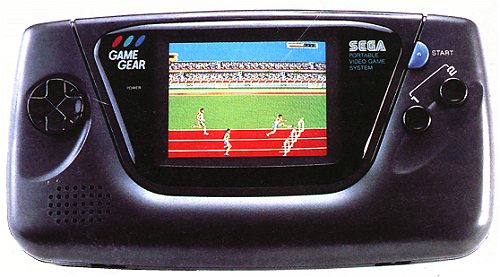
\includegraphics[scale=0.4]{gamegear.png}
\caption{Sega Game Gear \protect\cite{gg}}
\label{fig:gg}
\end{figure}

The image below shows a picture of internal PCB of the Game Gear and
it's major components

\begin{table}[H]
    \centering
    \begin{tabular}{|c|l|c|l|}
        \hline
        1 & Zilog Z80 CPU           & 4 & 16K VRAM      \\ \hline
        2 & Video Display Processor & 5 & Sega BIOS ROM \\ \hline
        3 & 8K RAM                  & 6 & Controller IO \\
        \hline
    \end{tabular}
\end{table}

\newpage
\subsection{Functional Diagrams}

At a high level the Game Gear can be viewed simply as a system which
takes input from a game controller and produces video and audio has an
output. This description is shown in Figure ~\ref{fig:external}

\begin{figure}[H]
\centering
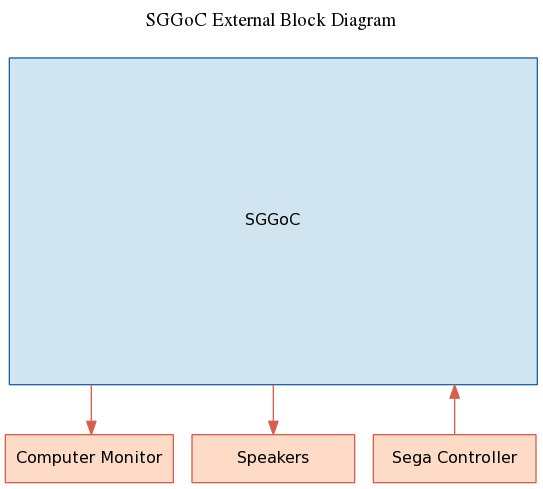
\includegraphics[scale=0.4]{../block_diagrams/block_diagram_external.png}
\caption{Black Box Diagram}
\label{fig:external}
\end{figure}

Internally the functionality can be easily modularized based on the
actual physical components. Additional components will be needed such
as an IO controller and a memory management unit (MMU) to account for 
the lack of tri-state buses in our design (explained later). Figure
~\ref{fig:internal} shows the major functional components in our
design and their interaction with each other.

\begin{figure}[H]
\centering
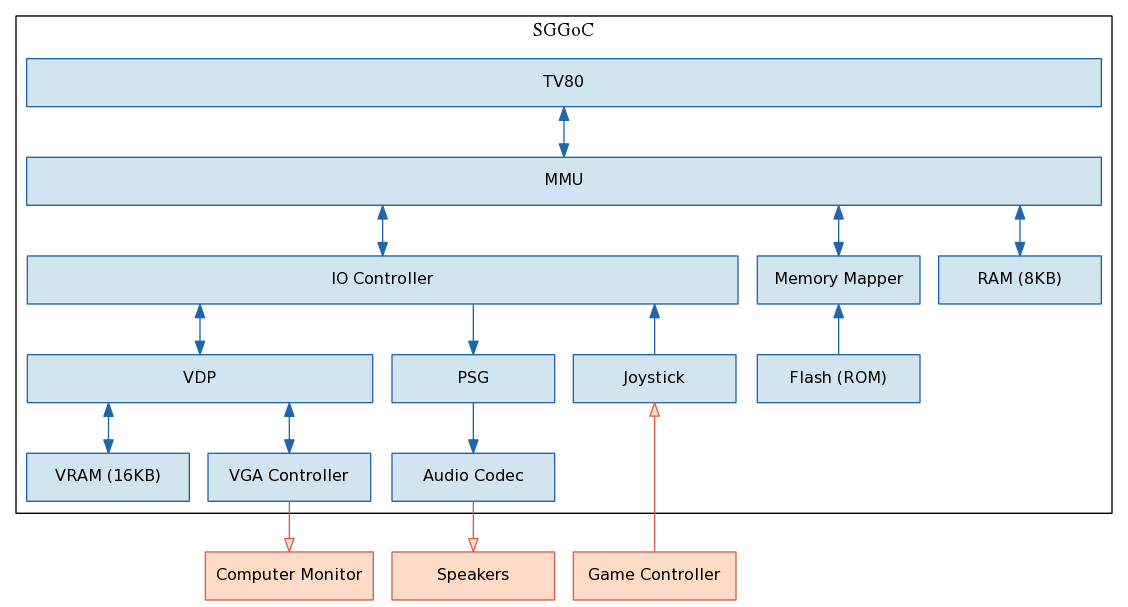
\includegraphics[scale=0.4]{../block_diagrams/block_diagram_internal.png}
\caption{Internal Functional Diagram}
\label{fig:internal}
\end{figure}

\newpage
\section{Cartridges and Memory Mapping}

The Z80 CPU only has 64KB of address space and only 48KB of it is
dedicated to the game cartridge. A "mapper" is used to allow the use of
larger ROMs (as well as on-catridge RAM). Figure ~\ref{fig:gg_cart}
shows a standard GG cartridge and Figure ~\ref{fig:gg_cart_pcb} shows
the internal PCB. The top chip is the Memory Mapper and the bottom chip
is the actual game ROM.

\begin{figure}[H]
    \centering
    \begin{minipage}[H]{0.3\linewidth}
        \centering
        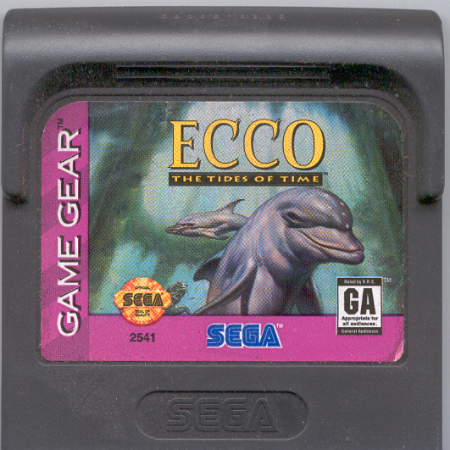
\includegraphics[width=\textwidth]{gg_cart.png}
        \caption{GG Cartridge\protect\cite{gg_cart}}
        \label{fig:gg_cart}
    \end{minipage}
    \hspace{1.5cm}
    \begin{minipage}[H]{0.3\linewidth}
        \centering
        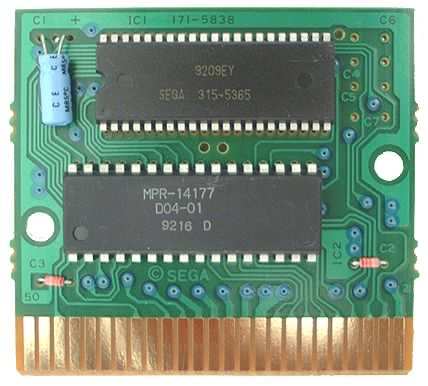
\includegraphics[width=\textwidth]{gg_cart_pcb.png}
        \caption{Cartridge PCB \protect\cite{gg_cart_pcb}}
        \label{fig:gg_cart_pcb}
    \end{minipage}
\end{figure}

\subsection{Sega Mapper}
There are several different mappers in existence but we will only
focus on implementing the "Sega Mapper" as it is the most popular.
The Sega mapper defines 3 16KB slots in the Z80 memory map. Any 16KB bank
of ROM can be mapped into any of these 3 slots. The mapping is
controlled by memory addresses 0xFFFC-0xFFFF.

\begin{table}[H]
    \centering
    \begin{tabular}{|c|c|c|}
        \hline
        \textbf{Control Register} & \textbf{Slot}     & \textbf{Maps to Z80 Address} \\ \hline
        0xFFFC           & Control Bits & -              \\ \hline
        0xFFFD           & 0            & 0x0000-0x3FFF  \\ \hline
        0xFFFE           & 1            & 0x4000-0x7FFF  \\ \hline
        0xFFFF           & 2            & 0x8000-0xBFFF  \\
        \hline
    \end{tabular}
    \caption{Mapper control registers \protect\cite{mapper}}
\end{table}

The ROM is viewed as an array of 16KB banks. The value written into 
the control register determines which bank is selected for 
that slot. Figure ~\ref{fig:mapping_diagram} shows an example of 
how the address space gets mapped to different ROM banks.

\begin{figure}[H]
\centering
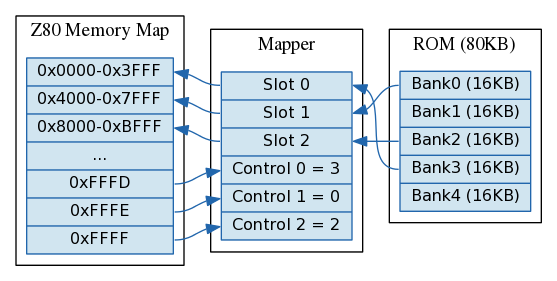
\includegraphics[scale=0.4]{mapper.png}
\caption{Mapping Diagram}
\label{fig:mapping_diagram}
\end{figure}

\subsection{Cartridge Alternatives}
Since we are targeting a standard FPGA development board we cannot
easily use the actual game cartridge without some kind of hardware adaptor.
Additionally, using the actual game cartridge would go
against what we are trying to accomplish with this project which is
eliminating the need for any of the original hardware. Lucky, virtually
every Game Gear cartridge has been dumped and are available online.
Unfortunately, the ROMs range in size all the way up to 4MB and being that
most affordable FPGAs do not have that much block RAM it would be
impossible for us to pack the ROM with the bitstream. A more ideal
solution would be to use a SD card which can be loaded with numerous
ROM files and then write a bootloader to select which one to play.
The complexity of that strategy, however, is not worth the initial
effort. A simpler solution which would allow us to quickly start on the
rest of the project is to load a single ROM file onto the Flash chip
that comes with our DE-1 development board.

\subsection{ROM Flasher}
The technical requirements of interfacing with the flash chip on our board
are outside the scope of our project and as such we will be using
a core provided by Altera \cite{flash_core} to simplify the process.
Figure ~\ref{fig:flash_core} shows the black box diagram of the flash core provided
by Altera.

\begin{figure}[H]
\centering
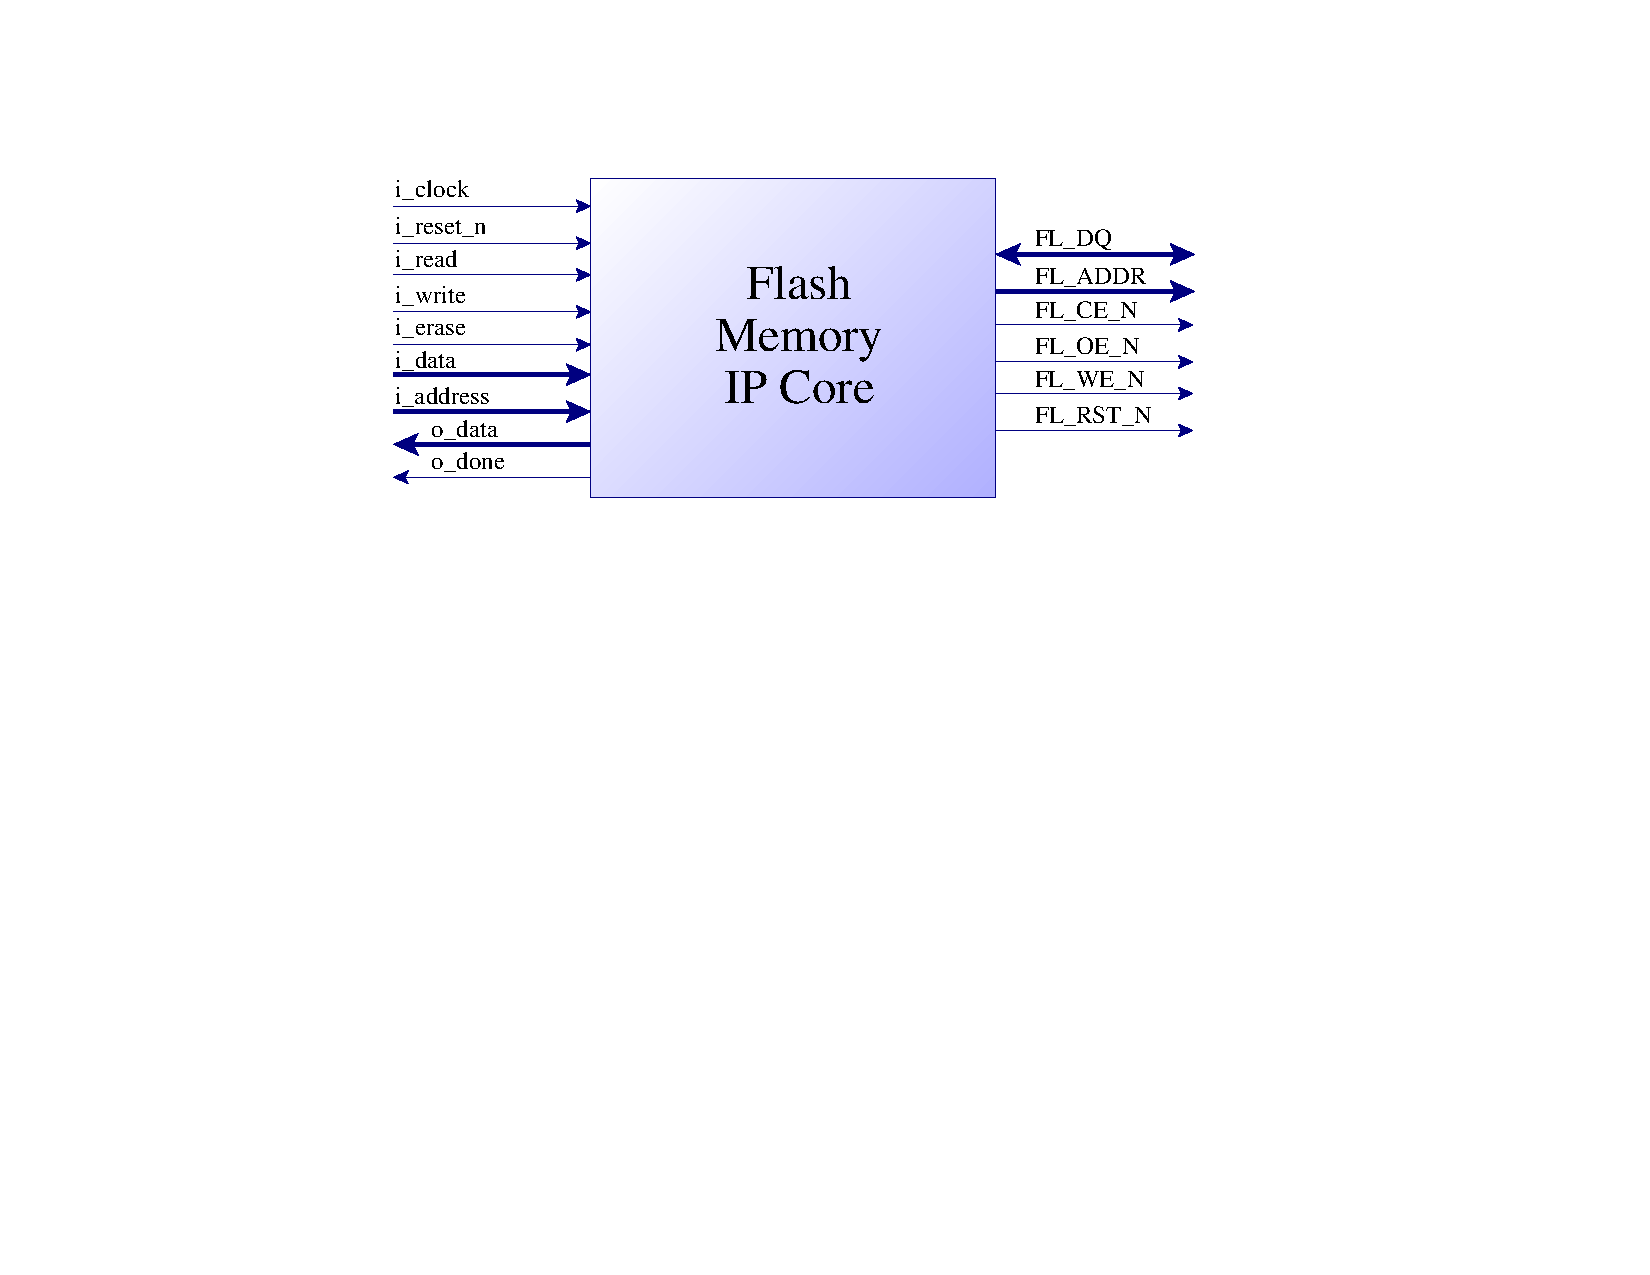
\includegraphics[scale=0.5]{flash_core.pdf}
\caption{Altera Flash Core}
\label{fig:flash_core}
\end{figure}

A "ROM Flasher" project, completely separate from the GG project,
will be used to initially load a single ROM file into the flash chip.
On the computer a Python program will read a ROM file byte by byte
and send it to the FPGA over the serial port. The FPGA will send back
the byte it just recieved as an acknowledgement. Another
Python program will be used to read back and verify that the flash contents
match the ROM file. Figures ~\ref{fig:rom_write} and ~\ref{fig:rom_read} 
illustrate the process of writing and reading a ROM to and from the
flash memory.

\begin{figure}[H]
    \centering
    \begin{minipage}[H]{0.45\linewidth}
        \centering
        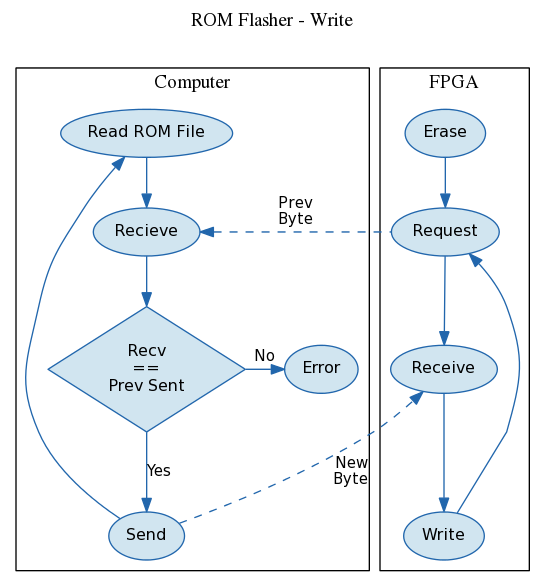
\includegraphics[width=\textwidth]{../../fpga/rom_flasher/doc/block_diagram_write.png}
        \caption{ROM Flasher - Write}
        \label{fig:rom_write}
    \end{minipage}
    \hspace{0.5cm}
    \begin{minipage}[H]{0.45\linewidth}
        \centering
        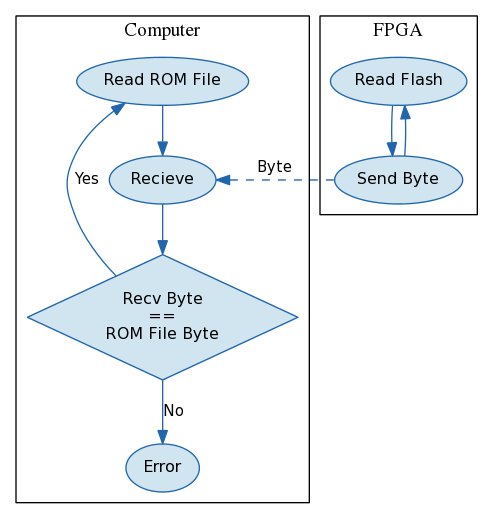
\includegraphics[width=\textwidth]{../../fpga/rom_flasher/doc/block_diagram_read.png}
        \caption{ROM Flasher - Read}
        \label{fig:rom_read}
    \end{minipage}
\end{figure}

\section{Zilog Z80}
The Game Gear uses the classic Zilog Z80 CPU running at 3.58MHz 
as it's main processor.
The re-implementation of the Z80 is completely outside the scope of
this project and as such we will be using the popular TV80 \cite{tv80}
CPU which is a proven, open source, implementation of the Z80
written in Verilog. The interface of the TV80 exactly matches that of
the original Z80, shown in Figure ~\ref{fig:z80}, with the only
exception being the data bus. The original Z80, as well as the whole
Game Gear memory system, relies on tri-state buses where as the TV80 has
a separate bus for data in and data out. 

\begin{figure}[H]
\centering
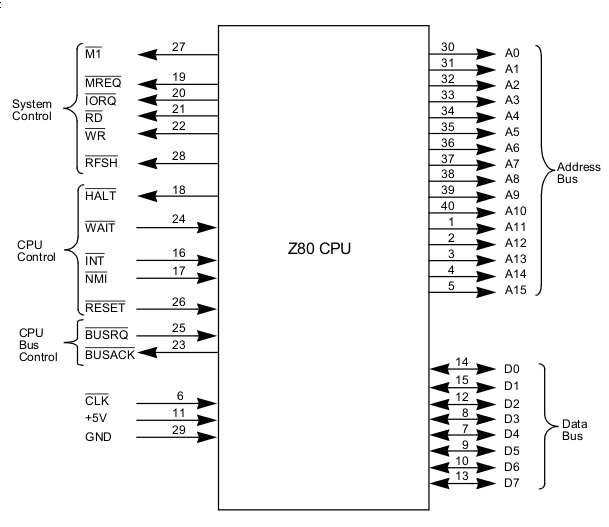
\includegraphics[scale=0.4]{z80.png}
\caption{Zilog Z80}
\label{fig:z80}
\end{figure}

\section{Memory Management Unit (MMU)}
Since our design does not use tri-state buses we cannot simply
connect the data lines from each component together. Instead, we
need to have some kind of memory manager that can multiplex the data
lines to whichever device the address is pointing to according the
system memory map. The full memory map for the Game Gear is shown below

\begin{table}[H]
    \centering
    \fontfamily{pcr}\selectfont
    \begin{tabular}{l|l}
        Address     & Device                           \\
        \hline
        \hline
        0x0000-0x03FF & ROM (unpaged)                    \\ 
        0x0400-0x3FFF & ROM mapper slot 0                \\ 
        0x4000-0x7FFF & ROM mapper slot 1                \\ 
        0x8000-0xBFFF & ROM mapper slot 2 - OR - SaveRAM \\ 
        0xC000-0xDFFF & System RAM                       \\ 
        0xE000-0xFFFF & System RAM (mirror)              \\ 
        0xFFFC       & SaveRAM mapper control           \\ 
        0xFFFD       & Mapper slot 0 control            \\ 
        0xFFFE       & Mapper slot 1 control            \\ 
        0xFFFF       & Mapper slot 2 control            \\
    \end{tabular}
    \fontfamily{}\selectfont
    \caption{Z80 Memory Map \protect\cite{mem_map_table}}
\end{table}

Since the cartridge memory mapper handles the slot mapping itself we are
really only multiplexing between the cartridge and the system RAM.
The system RAM happens to start at a nice edge being that
0xC000 = 0b1100000000000000. To see if we are accessing RAM
we only need to check to see if bits 15 and 16 are high. If so
we can simply use the 13 LSBs of the Z80 address as the index into the RAM. 
This method also accounts for the RAM mirror since the 13 LSBs repeat
starting at 0xE000.

\section{IO Controller}
\section{Video Display Processor (VDP)}

The Video Display Processor is a graphics chip which is derived from 
Texas Instruments (TMS9918). 

\subsection{Ports}

The VDP is accessed at the following Z80 I/O ports:

\begin{table}[H]
    \centering
    \begin{tabular}{c|p{3in}}
        \hline
        \hline
          \$7E & V counter (read) / SN76489 data (write)             \\ 
          \$7F & H counter (read) / SN76489 data (write, mirror)     \\ 
          \$BE & Data port (r/w)                                     \\ 
          \$BF & Control port (r/w)                                  \\
    \end{tabular}
\end{table}

The address decoding for the I/O ports is done with A7, A6 and A0
of the Z80 address bus, so the VDP locations are mirrored:

\begin{itemize}
    \item \$40 - 7F = Even locations are V counter/PSG, odd locations are H counter/PSG
    \item \$80 - BF = Even locations are data port, odd locations are control port.
\end{itemize}

%The H and V counters are described in the display timing section. The control 
%and data ports are des

\subsection{Control port}

The VDP is programmed by sending a two-byte sequence to the control port. The
control port is used to define an offset into VRAM or CRAM for subsequent data
port I/O, and also to write to the internal VDP registers.                          
\\

There is a flag which is set after the first byte is sent and cleared when
the second byte is written. This insures the VDP to know which byte of the
control port is being received. Note that the flag is also cleared when the
control port is read, and when the data port is read or written. This is used
to initialize the flag to zero after it has been modified unpredictably, after
an interrupt routine has executed, for example.                                     
\\

The VDP has two components that are used for accessing CRAM and VRAM:

\begin{itemize} 
    \item address register
    \item code register
\end{itemize}

The address register is 14 bits in length and defines the address into VRAM
for reads and writes, and the address into CRAM for writes. The code register
is 2 bits in length and selects four different operations:

\begin{itemize} 
    \item VRAM write
    \item VRAM read
    \item CRAM write
    \item VDP register write
\end{itemize}

The control port has the following format:

\begin{figure}[H]
    \centering
    \begin{bytefield}[bitwidth=2em, endianness=big]{8}
        \bitheader{0-7} \\
        \begin{rightwordgroup}{First Byte Written}
            \bitbox{1}{\tiny A07} & \bitbox{1}{\tiny A06} & \bitbox{1}{\tiny A05} & \bitbox{1}{\tiny A04} &
            \bitbox{1}{\tiny A03} & \bitbox{1}{\tiny A02} & \bitbox{1}{\tiny A01} & \bitbox{1}{\tiny A00}
        \end{rightwordgroup}\\
        \bitheader{0-7} \\
        \begin{rightwordgroup}{Second Byte Written}
            \bitbox{1}{\tiny CD1} & \bitbox{1}{\tiny CD0} & \bitbox{1}{\tiny A13} & \bitbox{1}{\tiny A12} & 
            \bitbox{1}{\tiny A11} & \bitbox{1}{\tiny A10} & \bitbox{1}{\tiny A09} & \bitbox{1}{\tiny A08} 
        \end{rightwordgroup}
    \end{bytefield}                                                                                                     
    \caption{Caption Here}
    \label{fig:figure1234}
\end{figure}

%\begin{table}[H]
%    \centering
%    %\begin{tabular}{@{\extracolsep{\fill}}|l|l|}
%    %\begin{tabular}{|@{}l@{}|@{}l@{}|}
%    \begin{tabular}{|l|l|}
%        \hline
%        %MSB \multicolumn{1}{|r|}{LSB} \\ \hline
%        MSB LSB                                                 \\ \hline
%        CD1 CD0 A13 A12 A11 A10 A09 A08 & Second byte written   \\ \hline
%        A07 A06 A05 A04 A03 A02 A01 A00 & First byte written    \\ 
%        \hline
%    \end{tabular}
%\end{table}

\begin{table}[H]
    \centering
    \begin{tabular}{l|l}
        \hline
        \hline
        CDX & Code register     \\ 
        AXX & Address register  \\
    \end{tabular}
\end{table}

When the first byte is written, the lower 8 bits of the address register are
updated. When the second byte is written, the upper 6 bits of the address
register and the code register are updated, and the VDP may carry out
additional processing based on the value of the code register:

\begin{table}[H]
    \centering
    \begin{tabular}{c|p{5in}}
        %\hline
        Code value      & Actions taken                                                 \\ 
        \hline
        \hline
            0           & A byte of VRAM is read from the location defined by           
                        the address register and is stored in the read buffer.        
                        The address register is incremented by one. Writes to         
                        the data port go to VRAM.                                     \\ 
            1           & Writes to the data port go to VRAM                            \\
            2           & This value signifies a VDP register write, explained below.   
                          Writes to the data port go to VRAM.                           \\
            3           & Writes to the data port go to CRAM.                           \\
    \end{tabular}
\end{table}


When accessing CRAM, the upper bits of the address register are ignored as CRAM
is smaller than 16k (either 32 or 64 bytes depending on the VDP). The address
register will wrap when it exceeds \$3FFF.                                      \\

\textbf{VDP register write}                                                     \\

While the address and code register are updated like normal when a VDP register
write is done, the control port sent can be viewed as having a different format
to the programmer: 

\begin{figure}[H]
    \centering
    \begin{bytefield}[bitwidth=2em, endianness=big]{8}
        \bitheader{0-7} \\
        \begin{rightwordgroup}{First Byte Written}
            \bitbox{1}{\tiny D07} & \bitbox{1}{\tiny D06} & \bitbox{1}{\tiny D05} & \bitbox{1}{\tiny D04} &
            \bitbox{1}{\tiny D03} & \bitbox{1}{\tiny D02} & \bitbox{1}{\tiny D01} & \bitbox{1}{\tiny D00}
        \end{rightwordgroup}\\
        \bitheader{0-7} \\
        \begin{rightwordgroup}{Second Byte Written}
            \bitbox{1}{\tiny 1}   & \bitbox{1}{\tiny 0}   & \bitbox{1}{\tiny X}   & \bitbox{1}{\tiny X} & 
            \bitbox{1}{\tiny R03} & \bitbox{1}{\tiny R02} & \bitbox{1}{\tiny R01} & \bitbox{1}{\tiny R00} 
        \end{rightwordgroup}
    \end{bytefield}                                                                                                     
    \caption{Caption Here}
    \label{fig:figure1234}
\end{figure}

%\begin{table}[H]
%    \centering
%    \begin{tabular}{|l|l|}
%        \hline
%        MSB LSB                                                 \\ \hline
%        1   0   ?   ?   R03 R02 R01 R00 & Second byte written   \\ \hline
%        D07 D06 D05 D04 D03 D02 D01 D00 & First byte written    \\ 
%        \hline
%    \end{tabular}
%\end{table}

\begin{table}[H]
    \centering
    \begin{tabular}{l|l}
        \hline
        \hline
        RXX & VDP register number   \\ 
        DXX & VDP register data     \\ 
         X  & Ignored               \\
    \end{tabular}
\end{table}

The VDP selects a register using bits 3-0 of the second byte, and writes the
data from the first byte to the register in question. There are only 10 registers, 
values 11 through 15 have no effect when written to.                                
\\

\textbf{Data Port}

Depending on the code register, data written to the data port is sent to either
VRAM or CRAM. After each write, the address register is incremented by one, and
will wrap past \$3FFF.                                                              
\\

Reads from VRAM or CRAM are buffered. Every time the data port is read (regardless
of the code register) the contents of a buffer are returned. The VDP will then
read a byte from VRAM at the current address, and increment the address register.
In this way data for the next data port read is ready with no delay while the
VDP reads VRAM. An additional quirk is that writing to the data port will also
load the buffer with the value written. 

\subsection{Status Flags}

Reading the control port returns a byte containing status flags:

\begin{figure}[H]
    \centering
    \begin{bytefield}[bitwidth=2em, endianness=big]{8}
        \bitheader{0-7} \\
        \bitbox{1}{\tiny INT} & \bitbox{1}{\tiny OVR} & \bitbox{1}{\tiny COL} & \bitbox{1}{\tiny ---} &
        \bitbox{1}{\tiny ---} & \bitbox{1}{\tiny ---} & \bitbox{1}{\tiny ---} & \bitbox{1}{\tiny ---}
    \end{bytefield}                                                                                                     
    \caption{Caption Here}
    \label{fig:figure1234}
\end{figure}

%\begin{table}[H]
%    \centering
%    \begin{tabular}{|l|}
%        \hline
%        MSB LSB                         \\ \hline
%        INT OVR COL --- --- --- --- --- \\ 
%        \hline
%    \end{tabular}
%\end{table}

\textbf{INT - Frame Interrupt Pending}                                  
\\

This flag is set on the first line after the end of the active display 
period.  It is cleared when the control port is read. (Please see the 
interrupts section for more details).                                   
\\

\textbf{OVR - Sprite Overflow}
\\

This flag is set if there are more than eight sprites that are positioned
on a single scanline. It is cleared when the control port is read. 
(Please see the sprites section for more information).                  
\\

\textbf{COL - Sprite Collision}
\\

This flag is set if an opaque pixel from any two sprites overlap. It is 
cleared when the control port is read. (Please see the sprites section
for more information).                                                  
\\

The remaining bits are not set by the VDP.

\subsection{Color RAM (CRAM)}

In Game Gear mode, CRAM has been expanded to 32 words or
64 bytes. Each word defined a single color as shown below: 

\begin{table}[H]
    \centering
    \begin{tabular}{l c l}
        - & = & Unused          \\ 
        R & = & Red pixels      \\ 
        G & = & Green pixels    \\ 
        B & = & Blue pixels     \\
    \end{tabular}
\end{table}

There are a total of 4096 (2\^{}12) possible colors that can be used, but only
32 colors can be shown at any given time.                                       
\\

The address register now wraps past address \$003F. Writing to an even CRAM
address causes the data written to be stored in a latch, and writing to an 
odd CRAM address makes the VDP write the contents of the latch as well as
the new data from the CPU to the current CRAM entry. For example:

\begin{table}[H]
    \centering
    \fontfamily{pcr}\selectfont
    \begin{tabular}{p{1cm} p{1in} p{3.5in}}
        %\hline
        ld  &  hl, \$C000   & ; CRAM address \$0000                     \\
        rst &  10h          & ; Assume this functions sets VDP address  \\
        ld  &  a, \$FF      & ; Color data                              \\
        out &  (\$BE), a    & ; CRAM unchanged, latch = \$FF            \\
        ld  &  hl, \$C021   & ; CRAM address \$0021                     \\
        rst &  10h          & ; Set the address again                   \\
        ld  &  a, \$0F      & ; Color data                              \\
        out &  (\$BE), a    & ; CRAM word at \$0020 is now \$0FFF, 
                                and the data at \$0000 is unchanged.    \\
        %\hline
    \end{tabular}
    \fontfamily{}\selectfont
    %\caption{
\end{table}

Therefore, writing single bytes to even CRAM addresses will not modify CRAM.
You could write multiple times to even addresses. This allows the same 
latched color data to be written to multiple palette entries.

\subsection{Display Modes}

The TMS9918 has three bits which select different display modes called M1,
M2, and M3. Note that in the TMS9918 manual, there are only four modes 
documented:

\begin{table}[H]
    \centering
    \begin{tabular}{l c c l}
        Mode & 0 & - & Graphics I   \\
        Mode & 1 & - & Text         \\
        Mode & 2 & - & Graphics II  \\
        Mode & 3 & - & Multicolor   \\
    \end{tabular}
\end{table}

%\subsection{Tiles}
%\subsection{CRAM}
%\subsection{Layers}
%\subsection{Interrupts}
%\subsection{Display Timing}
\section{Programmable Sound Generator (PSG)}
\section{VGA Controller}

\newpage
\begin{thebibliography}{9}
    \bibitem{gg} \url{http://mo5.com/musee-machines-gamegear.html}
    \bibitem{gg_cart} \url{http://www.magisterrex.com/prodimages/EccoDolphinGameGear-h450.png}
    \bibitem{gg_cart_pcb} \url{http://www.smspower.org/Development/SMSPagingChips}
    \bibitem{mapper} \url{http://www.smspower.org/Development/Mappers}
    \bibitem{flash_core} \url{ftp://ftp.altera.com/up/pub/flash/altera_up_flash_memory.zip}
    \bibitem{tv80} \url{http://opencores.org/project,tv80}
    \bibitem{mem_map_table} \url{http://code.google.com/p/bizhawk/source/browse/trunk/BizHawk.Emulation/Consoles/Sega/SMS/MemoryMap.Sega.cs}
    \bibitem{VDP} \url{http://www.smspower.org/uploads/Development/msvdp-20021112.txt?sid=c8bdf72dd28a0a34eeedf5f7742ca62a}
\end{thebibliography}

\end{document}
